\documentclass[11pt]{article}
\usepackage{amsmath}
\usepackage{amssymb}
\usepackage{graphicx}
\usepackage{fancyhdr}
\usepackage{enumerate}
\usepackage{titlesec}
\usepackage{subcaption}
\usepackage[colorlinks=true,urlcolor=blue]{hyperref}

\titlespacing{\subsubsection}{0pt}{0pt}{0pt}

% No page numbers
%\pagenumbering{gobble}

% INFORMATION SHEET (DO NOT EDIT THIS PART) ---------------------------------------------
\newcommand{\addinformationsheet}{
\clearpage
\thispagestyle{empty}
\begin{center}
\LARGE{\bf \textsf{Information sheet\\CS246: Mining Massive Data Sets}} \\*[4ex]
\end{center}
\vfill
\textbf{Assignment Submission } Fill in and include this information sheet with each of your assignments.  This page should be the last page of your submission.  Assignments are due at 11:59pm and are always due on a Thursday.  All students (SCPD and non-SCPD) must submit their homework via Gradescope (\url{http://www.gradescope.com}). Students can typeset or scan their homework. Make sure that you answer each (sub-)question on a separate page. That is, one answer per page regardless of the answer length. Students also need to upload their code on Gradescope. Put all the code for a single question into a single file and upload it.  
\\
\\
\textbf{Late Homework Policy } Each student will have a total of {\em two} late periods. {\em Homework are due on Thursdays at 11:59pm PT and one late period expires on the following Monday at 11:59pm PT}.  Only one late period may be used for an assignment.  Any homework received after 11:59pm PT on the Monday following the homework due date will receive no credit.  Once these late periods are exhausted, any assignments turned in late will receive no credit.
\\
\\
\textbf{Honor Code } We strongly encourage students to form study groups. Students may discuss and work on homework problems in groups. However, each student must write down their solutions independently, i.e., each student must understand the solution well enough in order to reconstruct it by him/herself.  Students should clearly mention the names of all the other students who were part of their discussion group. Using code or solutions obtained from the web (GitHub/Google/previous year's solutions etc.) is considered an honor code violation. We check all the submissions for plagiarism. We take the honor code very seriously and expect students to do the same. 
\vfill
}

% MARGINS (DO NOT EDIT) ---------------------------------------------
\oddsidemargin  0.25in \evensidemargin 0.25in \topmargin -0.5in
\headheight 0in \headsep 0.1in
\textwidth  6.5in \textheight 9in
\parskip 1.25ex  \parindent 0ex \footskip 20pt
% ---------------------------------------------------------------------------------

% HEADER (DO NOT EDIT) -----------------------------------------------
\newcommand{\problemnumber}{0}
\newcommand{\myname}{name}
\newfont{\myfont}{cmssbx10 scaled 1000}
\pagestyle{fancy}
\fancyhead{}
\fancyhead[L]{\myfont Question \problemnumber, Homework 1, CS246}
%\fancyhead[R]{\bssnine \myname}
\newcommand{\newquestion}[1]{
\clearpage % page break and flush floats
\renewcommand{\problemnumber}{#1} % set problem number for header
\phantom{}  % Put something on the page so it shows
}
% ---------------------------------------------------------------------------------


% BEGIN HOMEWORK HERE
\begin{document}

% Question 1
\newquestion{1}
\\ 
There are four steps that have been followed in the following implementation, in order to implement the "people you might know" solution in PySpark. Our solution uses pyspark dataframes. \\ \newline
\textbf{Step 1: Generate all indirect connections (A $\Rightarrow$ C) via common friends (A $\Rightarrow$ B $\Rightarrow$ C) by calculating all combinations of each person's 'B' connections}\\
In this step, we first iterate to the friends of a person 'B' and generate tuples between all of the person's friends. These persons have one common friend 'B', therefore
they can form a possible recommendation for a friend request. The cartessian product is calculated using the 'explode' function in the connection list, in PySpark, for two separate columns.
This will generate all possible pairs of friends of each person.\\ 
\newline

 \textbf{Step 2: Remove existing direct connections from the possible recommendations}\\
    In this step, we remove all the indirect connections that appear more than once, from the possible recommendations generated in Step 1. \\
    \newline

\textbf{Step 3: Count the quantity for each possible mutual friends recommendation}\\
    In this step, we group the possible indirect connections from the step 2 and count the quantity of each possible connection. This will give us 
    the number of mutual friends for each possible pair of people who are not direct friends.
\newline 

\textbf{Step 4: Normalise the table so each row becomes person $|$ friend $|$ count}\\
    From the table that has been generated in the step 3, one person can appear either as the "person" or as the "friend" in the possible recommendation. This means that if we try to
    group by one of these columns, to get one person's recommendations, we will lose information, because for any row where the person appears in the other column, the row will be grouped
    with the other person's recommendations. This is why we need 
    to normalise the result, so each person appears as "person" in all her possible recommendation and than, after a grouping, the top K recommendationscan be correctly extracted. 
\newline

\textbf{Step 5: For each person, select the top K (K=10) recommended indirect connections based on the highest occurrence counts}\\
    In this step, we use window functions to select the top K (K=10) recommended indirect connections based on the highest occurrence counts. 


% Question 2(a)
\newquestion{2(a)}

The drawback of using Confidence in an association rule $A \to B$ (which measures $P(B|A)$) is that it ignores the overall frequency (or probability) of the consequent itemset B, denoted as $P(B)$ (or Support(B)).
This can lead to misleading interpretations of the strength of the association between A and B. For example, if itemset B is very common in the dataset, it may have a high confidence value even if there is no real association between A and B. 
In such cases, the high confidence value may simply reflect the overall popularity of itemset B rather than a meaningful relationship with itemset A. Therefore, relying solely on confidence can result in overestimating the significance of certain association rules.\\
\newline 

% Question 2(b)
\newquestion{2(b)}

\textbf{Confidence} Confidence is not symmetrical.\\
\textit{Counterexample:} The formula for Confidence is:$$\text{Confidence}(A \to B) = \frac{\text{Support}(A \cup B)}{\text{Support}(A)} = \frac{P(A \cap B)}{P(A)}$$If we reverse the rule to $B \to A$, the formula becomes:$$\text{Confidence}(B \to A) = \frac{\text{Support}(B \cup A)}{\text{Support}(B)} = \frac{P(B \cap A)}{P(B)}$$Since $P(A \cap B) = P(B \cap A)$, the measures are equal only if their denominators are equal, i.e., $P(A) = P(B)$.
\\ \newline \textbf{Lift} Lift is symmetrical.\\
\textit{Proof:} The formula for Lift is:$$\text{Lift}(A \to B) = \frac{\text{Support}(A \cup B)}{\text{Support}(A) \times \text{Support}(B)} = \frac{P(A \cap B)}{P(A) \times P(B)}$$If we reverse the rule to $B \to A$, the formula becomes:$$\text{Lift}(B \to A) = \frac{\text{Support}(B \cup A)}{\text{Support}(B) \times \text{Support}(A)} = \frac{P(B \cap A)}{P(B) \times P(A)}$$Since $P(A \cap B) = P(B \cap A)$, the measures are equal.\\
\\ \newline \textbf{Conviction} Conviction is symmetrical.\\
\textit{Proof:} The formula for Conviction is:$$\text{Conviction}(A \to B) = \frac{P(A)}{1 - P(B|A)}$$If we reverse the rule to $B \to A$, the formula becomes:$$\text{Conviction}(B \to A) = \frac{P(B)}{1 - P(A|B)}$$Since $P(A \cap B) = P(B \cap A)$, the measures are equal.\\


% Question 2(c)
\newquestion{2(c)}

\textbf{Confidence} and \textbf{Conviction} are desirable. \textbf{Lift} is not.\\ \newline
\textit{Proof:}\\
\begin{itemize}
    \item \textbf{Confidence:} For a perfect implication ($P(B|A)=1$), Confidence reaches its maximum value of 1.
    \item \textbf{Conviction:} For a perfect implication, the denominator $1 - P(B|A)$ becomes 0, so Conviction reaches its maximum value of $\infty$.
    \item \textbf{Lift:} For a perfect implication, Lift equals $\frac{1}{P(B)}$. This value depends on the support of B and does not reach a constant maximum (like $\infty$) for all perfect implications.
\end{itemize}


% Question 2(d)
\newquestion{2(d)}

The top 5 association rules by confidence are:
\begin{itemize}
    \item DAI93856 $\to$ FRO40251
    \item GRO85051 $\to$ FRO40251
    \item GRO38636 $\to$ FRO40251
    \item ELE12951 $\to$ FRO40251
    \item DAI88079 $\to$ FRO40251
\end{itemize}
% Question 2(e)
\newquestion{2(e)}

The top 5 association rules between three items, by confidence are:
\begin{itemize}
    \item ('SNA18336', 'DAI62779') $\to$ 'ELE92920'
    \item ('DAI23334', 'DAI62779') $\to$ 'ELE92920'
    \item ('FRO92469', 'FRO40251') $\to$ 'SNA80324'
    \item ('GRO85051', 'FRO40251') $\to$ 'SNA80324'
    \item ('FRO47962', 'DAI75645') $\to$ 'GRO73461'
\end{itemize}   

% Question 3(a)
\newquestion{3(a)}

The total number of ways to get k rows out of n is given by the binomial coefficient $\binom{n}{k} = \frac{n!}{k!(n-k)!}$.  \newline 
The number of different ways to choose $k$ rows out of $n$, such that they all contain 0 (avoiding the $m$ rows with 1s) is
given by $\binom{n-m}{k}$. Thus, the probability of getting a partition of all zeros,out of all the possible partitions, is given by $\frac{\binom{n-m}{k}}{\binom{n}{k}}$. \newline 
By some simple calculations, the above quantity becomes 
$$ \frac{\binom{n-m}{k}}{\binom{n}{k}} = \frac{\frac{(n-m)!}{k!(n-m-k)!}}{\frac{n!}{k!(n-k)!}} = \frac{(n-m)!(n-k)!}{n!(n-m-k)!} = \frac{(n - k)(n - k - 1) ... }{n(n - 1) ... (n - k + 1)} = \prod_{i=0}^{m-1} \frac{n-k-i}{n-i}$$ 
We notice that as i increases, the quantity $\frac{n-k-i}{n-i}$ decreases. If we replace the quantity $\frac{n-k-i}{n-i}$ with the larger quantity $\frac{n-k}{n}$ for every $i$, we get a larger product.
Hence, we get the upper bound 
$$ \frac{\binom{n-m}{k}}{\binom{n}{k}} \leq \prod_{i=0}^{m-1} \frac{n-k}{n} = \left(\frac{n-k}{n}\right)^{m-1}$$
% Question 3(b)
\newquestion{3(b)}

Let's start from our desired property and work our wayto determine the minimum value of $k$ for which the probability is at least $e^{-10}$.

\begin{gather} 
    (\frac{n-k}{n})^m \leq e^{-10} \implies \\
    (1 - \frac{k}{n})^m \leq e^{-10} \implies \\
    m*ln(1 - \frac{k}{n}) \leq -10
\end{gather}

For very large $n$ and small $k$, the quantity $\frac{k}{n}$ becomes very small and closes to 0. Thus, we can use the Taylor series approximation for $ln(1 - x) \approx -x$. By using the Taylor series approximation on $(3)$, we 
can replace $ln(1 - \frac{k}{n})$ with $-\frac{k}{n}$. Therefore, the inequality becomes:

\begin{gather}
    m*(- \frac{k}{n}) \leq -10 \implies \\
    \frac{mk}{n} \geq 10 \implies \\
    k \geq \frac{10n}{m}
\end{gather}
 From the result in $(6)$, we can determine that the minimum value of $k$ for which the probability is at least $e^{-10}$ is $\frac{10n}{m}$.
% Question 3(c)
\newquestion{3(c)}

Let's assume that we have an example matrix with only three rows as follows:
\begin{gather}
    \begin{pmatrix}
        row & S_1 & S_2 \\
        0 & 1 & 0 \\
        1 & 1 & 1 \\
        2 & 0 & 1 \\
        3 & 0 & 0 
    \end{pmatrix}
\end{gather}

The Jaccard similarity between the two sets $S_1$ and $S_2$ is given by:
$$ J(S_1, S_2) = \frac{|S_1 \cap S_2|}{|S_1 \cup S_2|} = \frac{1}{3}$$

We have 4 possible cyclic permutations of the rows of the matrix. If we set the minhash value $h(S)$ to be the counter of the first 1 we encounter, then the minhash values for the 4 cyclic permutations are:

\begin{gather}
    \begin{pmatrix}
        permutation & row order & S_1 & S_2 \\
        0 & (0, 1, 2, 3) & 1 & 2 \\
        1 & (1, 2, 3, 0) & 1 & 1 \\
        2 & (2, 3, 0, 1) & 3 & 1 \\
        3 & (3, 0, 1, 2) & 2 & 3 
    \end{pmatrix}
\end{gather}
 In this case, the probability of the minhash values of the two columns being equal is $\frac{1}{4}$ (only in permutation 1).
% Question 4(a)
\newquestion{4(a)}

For this proof, we are going to start from the left part of the inequality that we want to proof correctly, and we will work our way out to transform it into the inequality at right. 
From the Markov inequality we have
\begin{gather}
    P_r[\sum_{j=1}^{L}{|T \cap W_{j}|} \geq 3L] \leq \frac{E[\sum_{j=1}^{L}{|T \cap W_{j}|}]}{3L}
\end{gather}
 For all the points $j$ we know that the probability of hashing at the same bucket, since $d(x,z) > c\lambda$ for all the points $j$ that belong to T, is at most $p_{2}$.
Given that, we can calculate the expected value of the sum as follows:
\begin{gather}
    E[\sum_{j=1}^{L}{|T \cap W_{j}|}] = \sum_{j=1}^{L}{E[|T \cap W_{j}|]} \le \sum_{j=1}^{L} |T| p_2 = L |T| p_2
\end{gather}
Combining the two inequalities 9 and 10 we get:
\begin{gather}
    P_r[\sum_{j=1}^{L}{|T \cap W_{j}|} \geq 3L] \leq \frac{L |T| p_{2}}{3L} = \frac{|T| p_{2}}{3}
\end{gather}
% Question 4(b)
\newquestion{4(b)}

Let $P$ be the probability that $g_j(x^*) = g_j(z)$ for a single hash function $g_j$ chosen from the family. Since $d(x^*, z) \le \lambda$ and the functions are locality sensitive, we have a certain collision probability $p$. For the standard construction using AND-families of $k$ primitive functions, $P \ge p_1^k$.
The probability that a single function $g_j$ fails to collide (i.e., $g_j(x^*) \neq g_j(z)$) is $1 - P$.
Since the $L$ functions in the family $g$ are chosen independently, the probability that all $L$ functions fail to collide is:
$$ \text{Pr}[\forall 1 \le j \le L, g_j(x^*) \neq g_j(z)] = (1 - P)^L $$
Using the inequality $1 - x \le e^{-x}$ (which is strict for $x > 0$), we have:
$$ (1 - P)^L < (e^{-P})^L = e^{-PL} $$
If we choose the parameter $L$ such that the expected number of collisions is at least 1 (i.e., $L \cdot P \ge 1$, or $L \ge 1/P$), then:
$$ e^{-PL} \le e^{-1} = \frac{1}{e} $$
Thus, proving that the probability of missing the neighbor $z$ is strictly less than $1/e$.

% Question 4(c)
\newquestion{4(c)}

From part 4(b), the probability that the approximate nearest neighbor $z$ is NOT found (false negative) is bounded by $1/e$.
From part 4(a), the probability that we retrieve more than $3L$ candidates from far points (false positives overload) is bounded by $1/3$ (assuming appropriate constants).
By the union bound, the probability that either we miss the neighbor OR we have too many false positives is at most $1/e + 1/3 \approx 0.368 + 0.333 \approx 0.7$.
Thus, with probability at least $1 - 0.7 = 0.3$ (a fixed constant $> 0$), the algorithm retrieves the neighbor $z$ and the number of other candidates to check is small ($< 3L$), allowing us to verify and report $z$ as an actual $(c, \lambda)$-ANN efficiently.


% Question 4(d)
\newquestion{4(d)}

In the matrix below, we present teh top-3 neighbors for each batch in rows 100,200,.. etc. for both the linear search and locality
sensitive hashing.
\begin{table}[h]
    \centering
    \begin{tabular}{|c|c|c|c|}
        \hline
        \textbf{Row} & \textbf{Linear Search} & \textbf{Locality Sensitive Hashing} \\ \hline
        100 & 7551, 8196, 28351 & 7551, 8196, 28351 \\ \hline
        200 & 91, 604, 1888 & 91, 604, 1888 \\ \hline
        300 & 22057, 10788, 8198 & 15818,  22057, 9006 \\ \hline
        400 & 41483, 3608, 3270 & 28676, 33010, 5875 \\ \hline
        500 & 1178, 557, 35904 & 1178, 557, 35904 \\ \hline 
        600 & 49309, 373, 44503 & 49309, 373, 44503 \\ \hline
        700 & 41352, 44006, 36422 & 41352, 44006, 36422 \\ \hline 
        800 & 30478, 44743, 34353 & 30478, 44743, 34353 \\ \hline 
        900 & 15184, 6585, 23588 & 15184, 6585, 23588 \\ \hline 
    \end{tabular}
    \caption{Top-3 neighbors for each batch in rows 100,200,.. etc. for both the linear search and locality sensitive hashing.}
    \label{tab:top3_neighbors}
\end{table}
It is obvious that the linear search method is more accurate but much slower than the locality sensitive hashing method. Approximately, linear search 
took 10 times more time to finish than the LSH. 

\begin{figure}[htbp]
    \centering
    \begin{minipage}{0.45\textwidth}
        \centering
        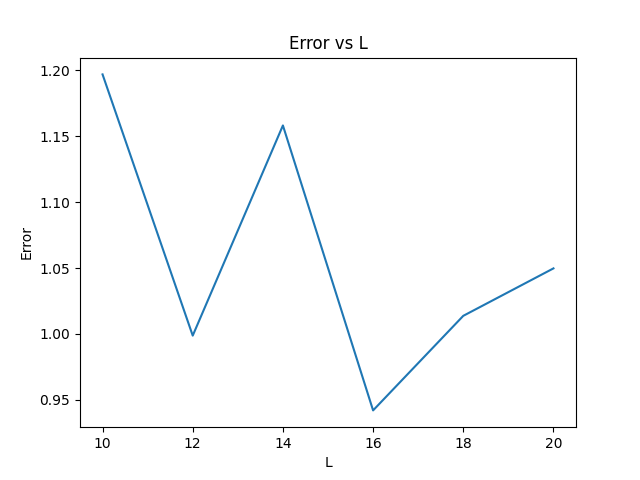
\includegraphics[width=\linewidth]{Figure_2.png}
    \caption{Error vs L}
    \label{fig:first}
    \end{minipage}\hfill
    \begin{minipage}{0.45\textwidth}
        \centering
        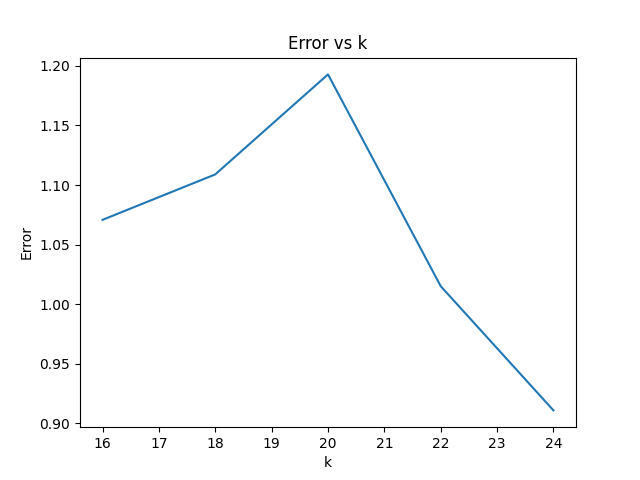
\includegraphics[width=\linewidth]{Figure_1.png}
    \caption{Error vs k}
    \label{fig:second}
    \end{minipage}
\end{figure}

The plots above show the error rate for different values of L and k. 
We can see that the error rate first increases and reaches a peak and then decreases as L and k increase. This is expected, as larger values of L and k increase the probability of finding the true nearest neighbor.

\begin{figure}[htbp]
    \centering
    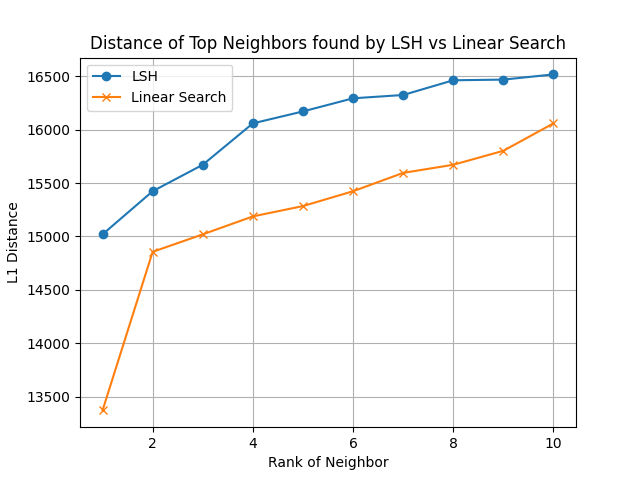
\includegraphics[width=\linewidth]{Figure_3.png}
    \caption{L1 distances of top 10 neighbors for linear search and LSH}
    \label{fig:third}
\end{figure}

The distances of the top 10 neighbors for linear search are generally lower than the distances of the top 10 LSH neighbors. This happens
because the linear search finds the 10 nearest neighbors, while the LSH finds the 10 nearest neighbors that are hashed to the same bucket. 
Notice that some of the neighbors have the exact same distance in both lines, which leads us to believe that it is the same neighbor. For instance,
the rank 3 of linear search and the rank 1 of LSH have the same distance of 22057, which is the 15818th instance of the dataset.





% Information sheet
% Fill out the information below (this should be the last page of your assignment)
\addinformationsheet
\vfill

{\Large
\textbf{Your name:} \hrulefill  % Put your name here
\\
\\
\textbf{Email:} \underline{\hspace*{7cm}}  % Put your e-mail here
\textbf{SUID:} \hrulefill  % Put your student ID here
\\*[2ex] 
}
Discussion Group: \hrulefill   % List your study group here
\\
\vfill\vfill
I acknowledge and accept the Honor Code.\\*[3ex]
\bigskip
\textit{(Signed)} 
\hrulefill   % Replace this line with your initials
\vfill






\end{document}
